\documentclass[pdftex,12pt,titlepage]{article}

\usepackage[pdftex]{graphicx}
\usepackage{amsfonts}
\usepackage{amsmath}
\usepackage{mychicago}
\usepackage{subfigure}
\usepackage{sidecap}
\usepackage{evolution_style}
\usepackage{xcolor}
\usepackage{float}
\usepackage[justification=raggedright]{caption}
\usepackage[subfigure]{tocloft} 
\usepackage{listings} 
\usepackage{fancyhdr}
\usepackage{rotating}
\usepackage[flushmargin,hang,multiple,ragged]{footmisc}

\date{}

% custom commands
\raggedbottom
\setlength{\headheight}{15pt}
\renewcommand{\headrulewidth}{0pt}
\newcommand{\ud}{\mathrm{d}}
\pagestyle{fancyplain}
\cfoot{\thepage}
\clubpenalty=10000
\widowpenalty=10000
\renewcommand{\tablename}{\textbf{Table}}
%\renewcommand{\figurename}{Figure}
\floatstyle{plain}
\DeclareCaptionLabelSeparator{emdash}{.---}
\DeclareCaptionLabelSeparator{mynewline}{\par\vspace{0.4cm}}
\DeclareCaptionLabelFormat{sformat}{#1~S#2}
\DeclareCaptionLabelFormat{tformat}{\textbf{#1~S#2}}
\captionsetup[figure]{labelsep=emdash,textfont=footnotesize,labelformat=sformat}
\captionsetup[table]{justification=centering,labelsep=mynewline,labelformat=tformat}

\begin{document}

\setlength{\parindent}{0cm}

\begin{center}
\large Supporting Information for:

\vspace{1cm}

\Large Multidimensional adaptive evolution of a feed-forward network and\\the illusion of compensation

\vspace{1cm}

\normalsize
Kevin Bullaughey

\vspace{1cm}

Dept. of Ecology \& Evolution, University of Chicago \\ 
920 E. 58th Street, CLSC 413\\ 
Chicago, IL 60637 \\ 
773-702-2750 (ph.)  773-834-0505 (fax)  \\ 

\texttt{bullaugh@uchicago.edu}
\end{center}

\raggedright
\hyphenpenalty10000
\clearpage

\setlength{\parindent}{1cm}
\begin{table}[p]
\caption{\textbf{Reversals during adaptation from random starting points using SMS approximation}}\label{smsTable}
\vspace{0.3cm}
\begin{center}
\begin{tabular}{c|c|c|c|c|c}
\hline
\hline
  & & \multicolumn{2}{c|}{\textbf{Forward portion}} & \multicolumn{2}{c}{\textbf{Reversal portion}} \\
\cline{3-6}
\textbf{Trait} & \textbf{Reversals}$^{a}$ 
  & \textbf{median} $s^{b}$ & \textbf{median} $\Delta^c$ 
  & \textbf{median} $s^{b}$ & \textbf{median} $\Delta^c$ \\
\hline
\hline
$\alpha_y$ & 100 & 0.83 & 0.63 & 0.08 & 0.17 \\ 
$\beta_y$  & 137 & 0.65 & 0.80 & 0.07 & 0.19 \\ 
$\alpha_z$ &   9 & 0.62 & 0.61 & 0.49 & 0.07 \\ 
$\beta_z$  &   0 &    - &    - &    - &    - \\ 
$k$        & 165 & 0.51 & 0.67 & 0.09 & 0.32 \\ 
\hline
\end{tabular}
\end{center}
\vspace{0.2cm}
$^{a}$\small{Reversals observed when evaluating the SMS model starting from 200 random starting points conditional on fitness $> 0$. Adaptation is in the high-noise environment. Only certain reversals are counted: reversals that involve a trait retracing at least 5\% of the average improvement in that trait and the largest observed reversal affecting each trait in each simulation (a few adaptive trajectories include multiple reversals affecting a single trait).}\\
$^{b}$\small{Median relative change in fitness during the reversal portion. Measured as $s = \frac{w_1}{w_0} - 1$ where $w_0$ is the absolute fitness at the beginning of the reversal portion and $w_1$ is the absolute fitness at the end of the reversal portion. Note that the fitness improvement is not due solely to the trait for which the reversal is observed, but is the combined fitness improvement due to changes in all traits during this portion of the multidimensional adaptive trajectory.}\\
$^{c}$\small{Median change in the trait observed over the reversal portion, normalized by average change across all runs.}\\
\end{table}
\clearpage

\begin{figure}[p]
\begin{center}
\resizebox{0.64\columnwidth}{!}{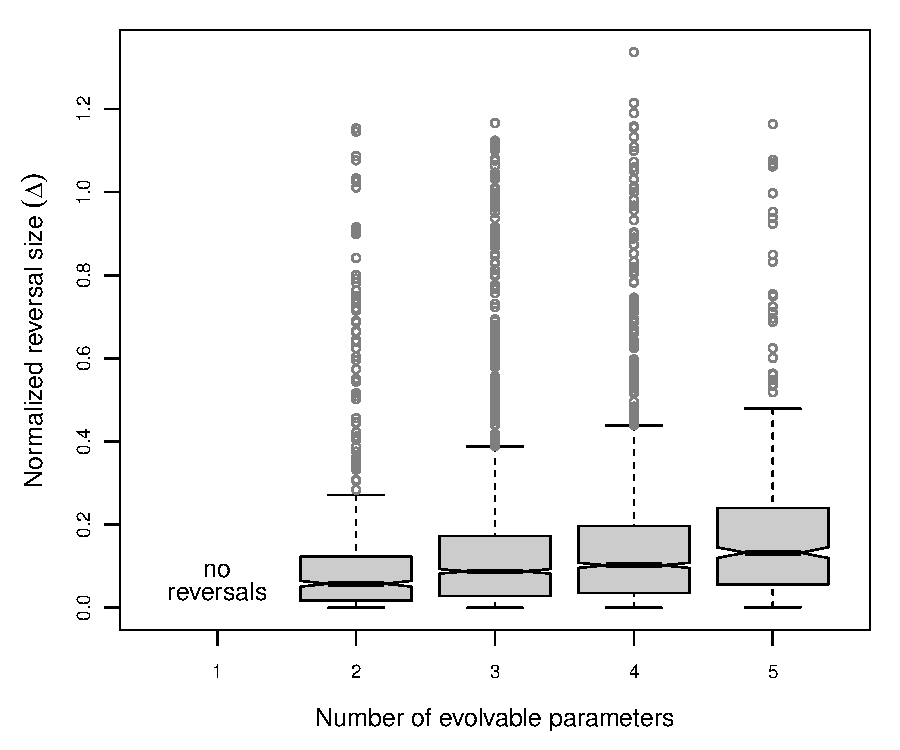
\includegraphics{suppfigs/reversal_sizes_by_dimension.pdf}}
%RevSizes
\caption{Size of reversals increases with dimensionality. This analysis involves the same data as in Figure 7. Briefly, evolution is restricted to subsets of the five traits and for each of the 31 non-empty subsets the adaptive trajectories for 200 random starting points are examined. Here, the normalized sizes (vertical axis) of the adaptive reversals are organized by the number of freely evolving traits (horizontal axis). The normalized reversal size is the amount the adaptive reversal retraces its path when projected onto one dimension and then normalized by the average change in the trait observed when all five traits are free to evolve. The boxplot is plotted in the standard way, with the bottom, middle, and top of the shaded gray areas are the 25\%, 50\%, and 75\% quantiles, with notches equal to the median $\pm\ 1.58 q/\sqrt{n}$. Where $q$ is the interquartile range and $n$ is the number of reversals identified. Whiskers extend 1.5 times the height of the shaded region and points beyond this are shown.}
\label{RevSizes}
\end{center}
\end{figure}
\clearpage

\end{document}

% END
